\documentclass[tikz,border=8pt]{standalone}

\usepackage[T1]{fontenc}
\usepackage{lmodern}
\usetikzlibrary{arrows.meta,backgrounds,calc,positioning,fit,shapes.geometric}

\definecolor{flowblue}{HTML}{0072B2}
\definecolor{flowgreen}{HTML}{009E73}
\definecolor{flowbrown}{HTML}{8C564B}
\definecolor{flowpurple}{HTML}{6F4EA1}
\definecolor{floworange}{HTML}{D55E00}
\definecolor{ink}{HTML}{243447}
\definecolor{mutedink}{HTML}{52606D}
\definecolor{linegray}{HTML}{9AA5B1}
\definecolor{panel}{HTML}{F5F7FA}
\definecolor{ownedfill}{HTML}{E8F1F8}
\definecolor{storefill}{HTML}{FFF1CC}
\definecolor{externalfill}{HTML}{F3ECF8}

\tikzset{
  box/.style={
    draw=linegray,
    fill=white,
    rounded corners=2pt,
    line width=0.6pt,
    minimum height=10mm,
    text width=30mm,
    align=center,
    font=\sffamily\small,
    text=ink,
    inner sep=4pt
  },
  actor/.style={box,text width=24mm},
  component/.style={box,fill=ownedfill},
  store/.style={box,fill=storefill,text width=24mm},
  external/.style={box,fill=externalfill,text width=34mm},
  network/.style={box,text width=26mm},
  boundary title/.style={font=\sffamily\bfseries\large,text=ink,anchor=west},
  flow/.style={-{Latex[length=3mm,width=2.2mm]},line width=1.6pt},
  story one/.style={flow,draw=flowblue},
  story two/.style={flow,draw=flowgreen},
  story three/.style={flow,draw=flowbrown},
  story four/.style={flow,draw=flowpurple},
  story five/.style={flow,draw=floworange},
  relation/.style={draw=linegray,line width=1.1pt},
  edge label/.style={
    fill=none,
    inner xsep=1.5pt,
    inner ysep=3pt,
    font=\sffamily\scriptsize,
    text=mutedink,
    align=center
  },
  every node/.append style={font=\sffamily}
}

\newcommand{\storyStep}[2]{%
  \tikz[baseline=(step.base)]
    \node[circle,fill=#1,text=white,inner sep=1.1pt,
      font=\sffamily\bfseries\tiny] (step) {#2};%
}


\tikzset{
  dependency/.style={relation,-{Latex[length=2.3mm,width=1.6mm]}},
  planned/.style={component,dashed,fill=white},
  smallbox/.style={component,text width=27mm,minimum height=10mm},
  table/.style={box,align=left,text width=50mm,inner sep=7pt,font=\sffamily\small},
  fk/.style={relation,-{Latex[length=2.6mm]},draw=ink,line width=1.2pt},
  logical/.style={relation,-{Latex[length=2.6mm]},draw=flowblue,dashed,line width=1.2pt},
  note/.style={font=\sffamily\small,text=mutedink,align=left},
  title/.style={font=\sffamily\bfseries\Large,text=ink,anchor=west}
}

\begin{document}
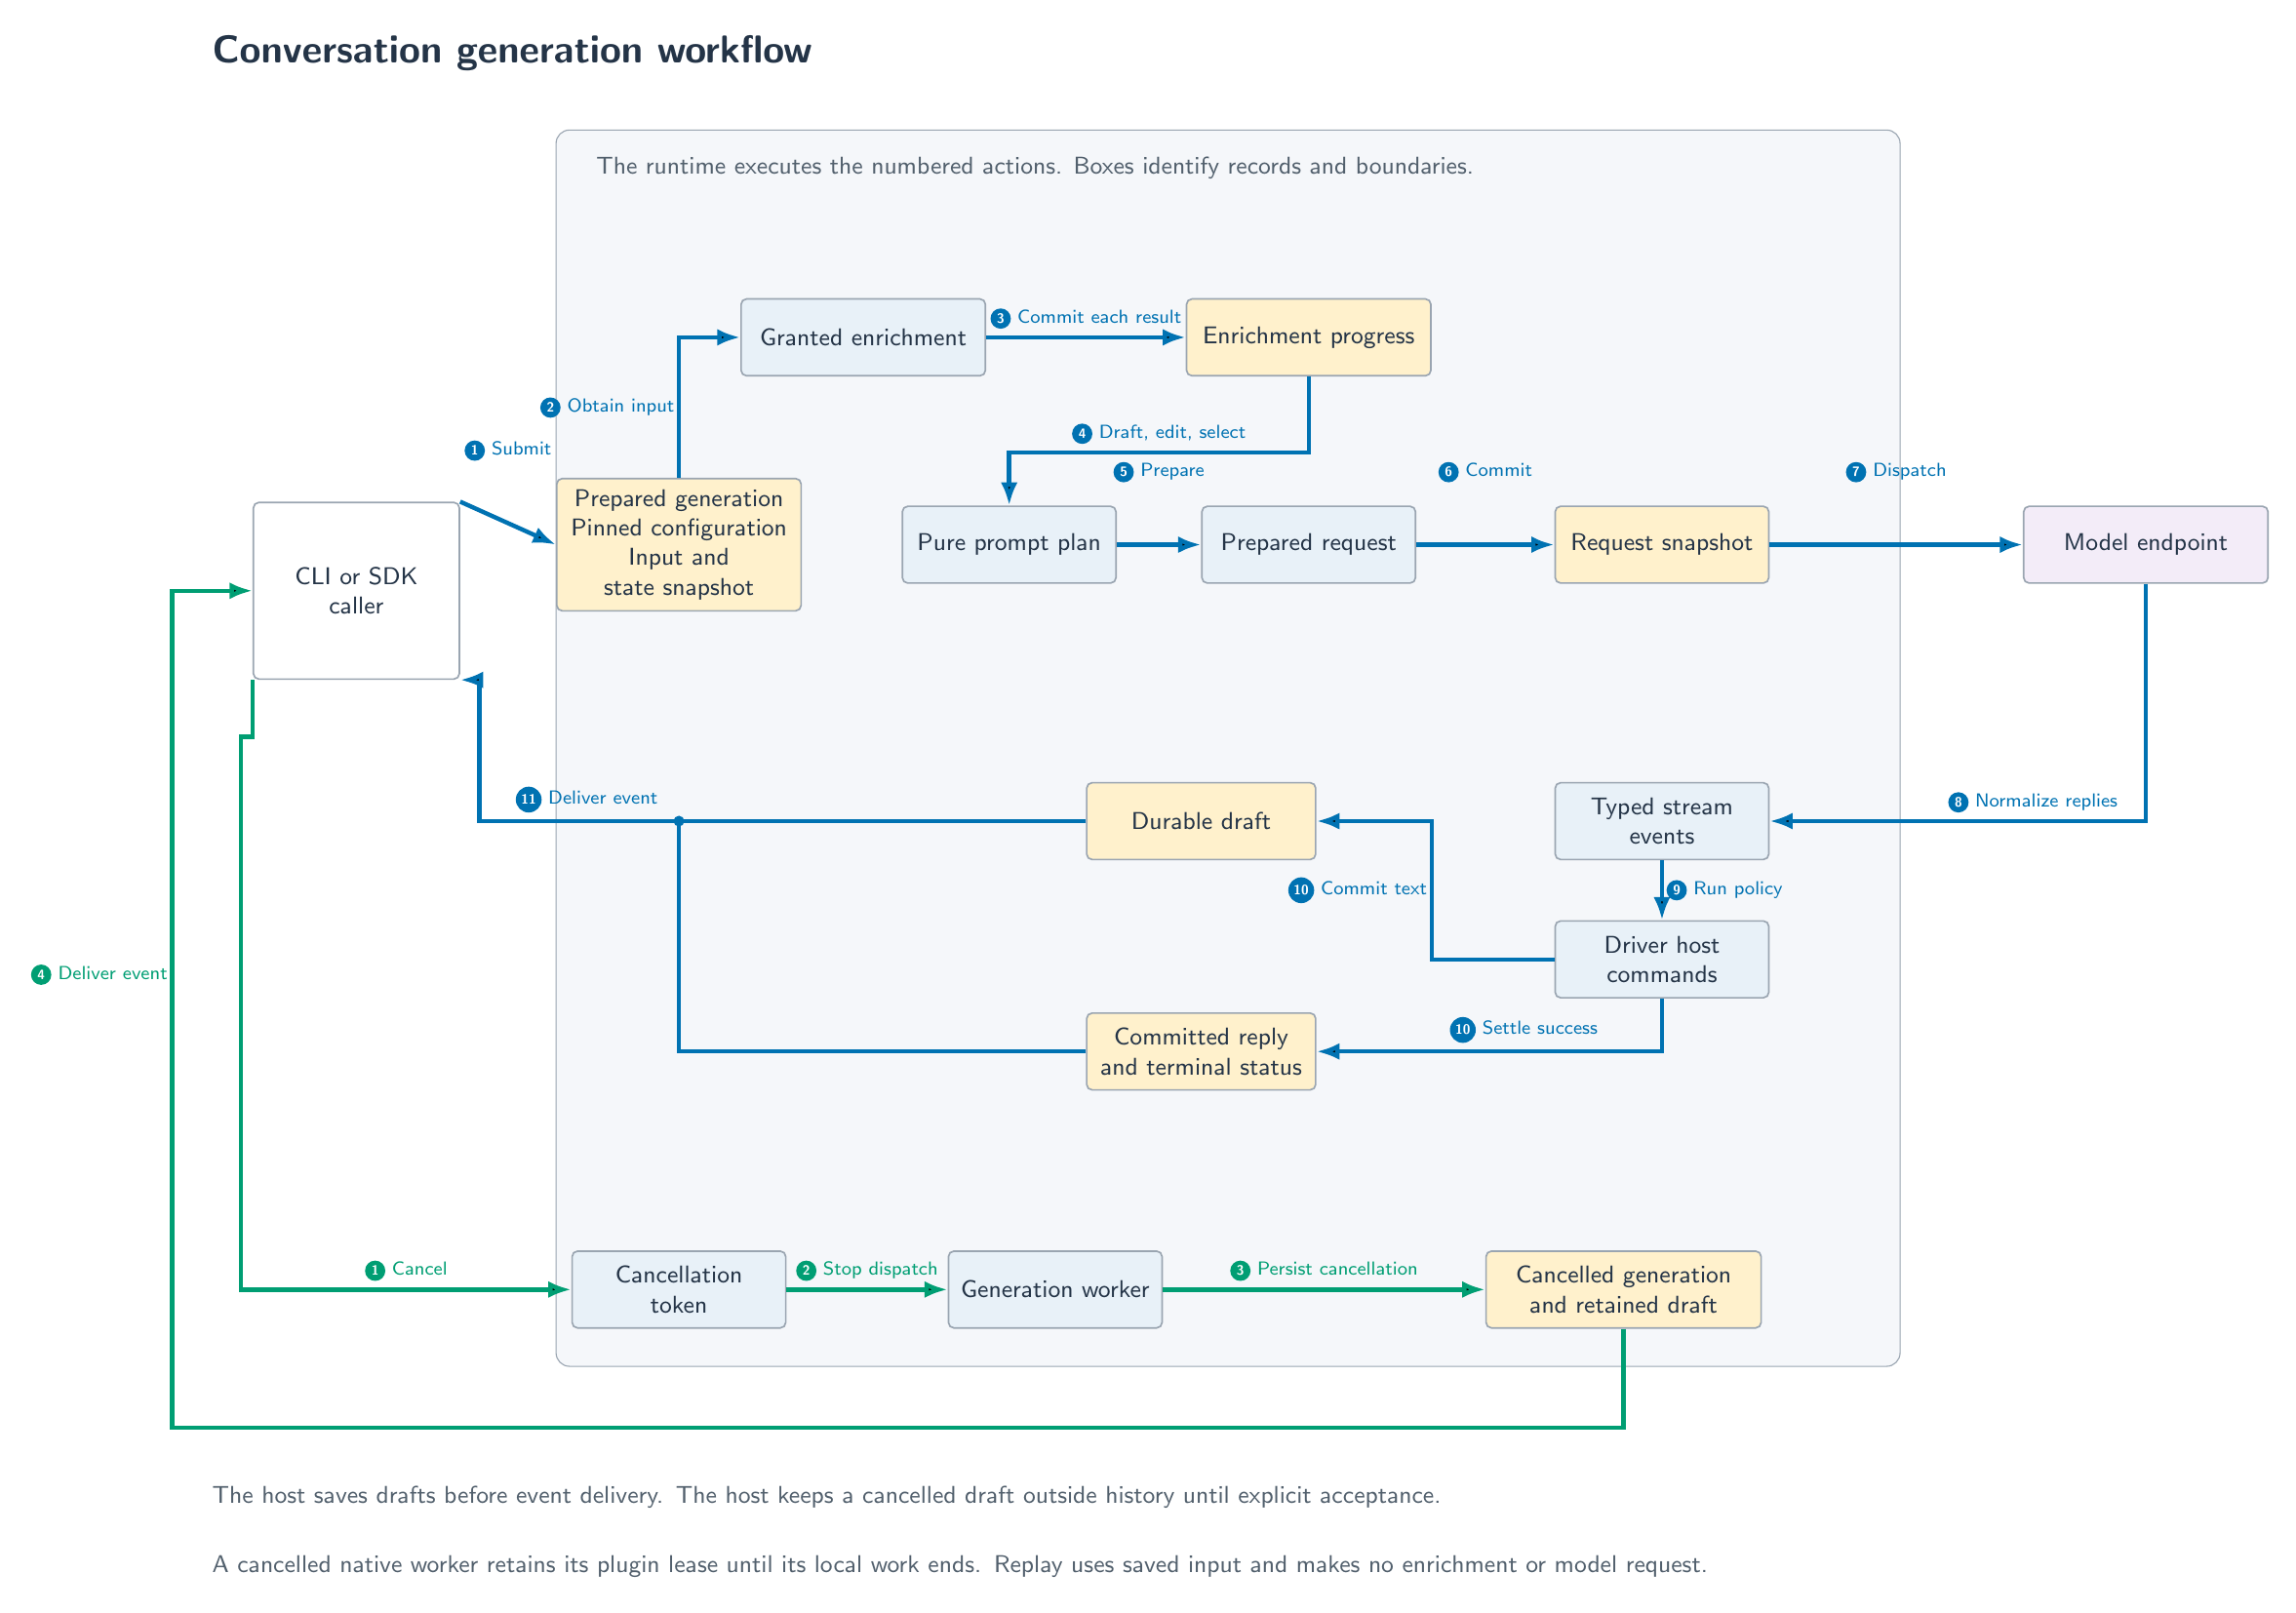
\begin{tikzpicture}[x=1cm,y=1cm]

\node[title] at (-2,15.7) {Conversation generation workflow};
\begin{scope}[on background layer]
  \filldraw[fill=panel,draw=linegray,rounded corners=5pt] (2.6,-1.4) rectangle (20.1,14.7);
\end{scope}
\node[note,anchor=west] at (3,14.2) {The runtime executes the numbered actions. Boxes identify records and boundaries.};
\node[actor,minimum height=23mm] (caller) at (0,8.7) {CLI or SDK\\caller};
\node[store,text width=29mm] (prepared) at (4.2,9.3) {Prepared generation\\Pinned configuration\\Input and state snapshot};
\node[component,text width=29mm] (enrichment) at (6.6,12) {Granted enrichment};
\node[store,text width=29mm] (enriched) at (12.4,12) {Enrichment progress};
\node[component,text width=25mm] (plan) at (8.5,9.3) {Pure prompt plan};
\node[component,text width=25mm] (request) at (12.4,9.3) {Prepared request};
\node[store,text width=25mm] (saved) at (17,9.3) {Request snapshot};
\node[external,text width=29mm] (model) at (23.3,9.3) {Model endpoint};
\node[component,text width=25mm] (events) at (17,5.7) {Typed stream\\events};
\node[component,text width=25mm] (driver) at (17,3.9) {Driver host commands};
\node[store,text width=27mm] (draft) at (11,5.7) {Durable draft};
\node[store,text width=27mm] (reply) at (11,2.7) {Committed reply\\and terminal status};
\coordinate (delivery) at (4.2,5.7);
\fill[flowblue] (delivery) circle (2pt);
\draw[story one] (caller.north east) -- node[edge label,above=7mm,text=flowblue] {\storyStep{flowblue}{1} Submit} (prepared.west);
\draw[story one] (prepared.north) -- node[edge label,left,text=flowblue] {\storyStep{flowblue}{2} Obtain input} (4.2,12) -- (enrichment.west);
\draw[story one] (enrichment.east) -- node[edge label,above,text=flowblue] {\storyStep{flowblue}{3} Commit each result} (enriched.west);
\draw[story one] (enriched.south) -- (12.4,10.5) -- node[edge label,above,text=flowblue] {\storyStep{flowblue}{4} Draft, edit, select} (8.5,10.5) -- (plan.north);
\draw[story one] (plan.east) -- node[edge label,above=7mm,text=flowblue] {\storyStep{flowblue}{5} Prepare} (request.west);
\draw[story one] (request.east) -- node[edge label,above=7mm,text=flowblue] {\storyStep{flowblue}{6} Commit} (saved.west);
\draw[story one] (saved.east) -- node[edge label,above=7mm,text=flowblue] {\storyStep{flowblue}{7} Dispatch} (model.west);
\draw[story one] (model.south) |- node[edge label,pos=.65,above,text=flowblue] {\storyStep{flowblue}{8} Normalize replies} (events.east);
\draw[story one] (events.south) -- node[edge label,right,text=flowblue] {\storyStep{flowblue}{9} Run policy} (driver.north);
\draw[story one] (driver.west) -- (14,3.9) -- (14,5.7) -- (draft.east);
\node[edge label,left,text=flowblue] at (14,4.8) {\storyStep{flowblue}{10} Commit text};
\draw[story one] (driver.south) |- node[edge label,pos=.7,above,text=flowblue] {\storyStep{flowblue}{10} Settle success} (reply.east);
\draw[story one,-] (draft.west) -- (delivery);
\draw[story one,-] (reply.west) -| (delivery);
\draw[story one] (delivery) -- (1.6,5.7) |- (caller.south east);
\node[edge label,above,text=flowblue] at (3,5.7) {\storyStep{flowblue}{11} Deliver event};
\node[component,text width=25mm] (cancel) at (4.2,-.4) {Cancellation token};
\node[component,text width=25mm] (consumer) at (9.1,-.4) {Generation worker};
\node[store,text width=33mm] (cancelled) at (16.5,-.4) {Cancelled generation\\and retained draft};
\draw[story two] (caller.south west) |- (-1.5,6.8) -- (-1.5,-.4) -- node[edge label,above,text=flowgreen] {\storyStep{flowgreen}{1} Cancel} (cancel.west);
\draw[story two] (cancel.east) -- node[edge label,above,text=flowgreen] {\storyStep{flowgreen}{2} Stop dispatch} (consumer.west);
\draw[story two] (consumer.east) -- node[edge label,above,text=flowgreen] {\storyStep{flowgreen}{3} Persist cancellation} (cancelled.west);
\draw[story two] (cancelled.south) -- (16.5,-2.2) -- (-2.4,-2.2) |- (caller.west);
\node[edge label,left,text=flowgreen] at (-2.4,3.7) {\storyStep{flowgreen}{4} Deliver event};
\node[note,anchor=west,text width=250mm] at (-2,-3.1) {The host saves drafts before event delivery. The host keeps a cancelled draft outside history until explicit acceptance.};

\node[note,anchor=west,text width=250mm] at (-2,-4) {A cancelled native worker retains its plugin lease until its local work ends. Replay uses saved input and makes no enrichment or model request.};

\end{tikzpicture}
\end{document}
